% AER-Article.tex for AEA last revised 22 June 2011
\documentclass[]{AEA}
\usepackage{amsmath}
\def\sym#1{\ifmmode^{#1}\else\(^{#1}\)\fi}
\usepackage{float} %設定圖片浮動位置的宏包
\usepackage{graphicx} %插入圖片
\usepackage{subfigure} %插入多圖時用子圖顯示
\usepackage{siunitx} % used for regression table
\usepackage{booktabs} % used for regression table
\usepackage{natbib}
\setcitestyle{authoryear, round}


%%%%%% NOTE FROM OVERLEAF: The mathtime package is no longer publicly available nor distributed. We recommend using a different font package e.g. mathptmx if you'd like to use a Times font.
% \usepackage{mathptmx}

% The mathtime package uses a Times font instead of Computer Modern.
% Uncomment the line below if you wish to use the mathtime package:
%\usepackage[cmbold]{mathtime}
% Note that miktex, by default, configures the mathtime package to use commercial fonts
% which you may not have. If you would like to use mathtime but you are seeing error
% messages about missing fonts (mtex.pfb, mtsy.pfb, or rmtmi.pfb) then please see
% the technical support document at http://www.aeaweb.org/templates/technical_support.pdf
% for instructions on fixing this problem.

% Note: you may use either harvard or natbib (but not both) to provide a wider
% variety of citation commands than latex supports natively. See below.

% Uncomment the next line to use the natbib package with bibtex 
%\usepackage{natbib}

% Uncomment the next line to use the harvard package with bibtex
%\usepackage[abbr]{harvard}

% This command determines the leading (vertical space between lines) in draft mode
% with 1.5 corresponding to "double" spacing.

\draftSpacing{1.5}

\begin{document}


\title{How does Single Parent Family Affect Children's Human Capital Investment}
\shortTitle{Single Parent family effect}
\author{Yi Jie Wu, Xiang Jyun Jhang\thanks{Wu: Department of Economics, National Taiwan University, b08302129@ntu.edu.tw; Jhang: Department of Economics, National Taiwan University, b08303024@ntu.edu.tw.  We are sincerely grateful for comments and advices from prof. Tzu-Ting Yang}}
\date{\today}
\pubMonth{JULY}
\pubYear{2023}

\begin{abstract}
    We estimate the impact of living in the single parent family on the children's future educational attainment by using a comprehensive panel survey data on students in Taiwan (TEPS).  By conducting PDS method, it's found that the experience of living under single parent family will decrease the probability of attaining university degree by 2.6 percent, and master degree by 4.6 percents also.  We also finds that there is a gap between the probability for two different groups of sample, which we provides some evidence to show it is attributed to the Taiwan Educational Reform in 2000s.
\end{abstract}


\maketitle

American Economic Review Pointers:

\begin{itemize}
\item Do not use an ``Introduction'' heading. Begin your introductory material
before the first section heading.

\item Avoid style markup (except sparingly for emphasis).

\item Avoid using explicit vertical or horizontal space.

\item Captions are short and go below figures but above tables.

\item The tablenotes or figurenotes environments may be used below tables
or figures, respectively, as demonstrated below.

\item If you have difficulties with the mathtime package, adjust the package
options appropriately for your platform. If you can't get it to work, just
remove the package or see our technical support document online (please
refer to the author instructions).

\item If you are using an appendix, it goes last, after the bibliography.
Use regular section headings to make the appendix headings.

\item If you are not using an appendix, you may delete the appendix command
and sample appendix section heading.

\item Either the natbib package or the harvard package may be used with bibtex.
To include one of these packages, uncomment the appropriate usepackage command
above. Note: you can't use both packages at once or compile-time errors will result.

\end{itemize}

\section{Data and Sample} % first paragraph: how the sample is built from the dataset?

    The dataset we use are Taiwan Education Panel Survey (TEPS) and Taiwan Education Panel Survey and Beyond (TEPS-B), in which there are two group of children being surveyed consistently from their schoold age (16-18) to their working age (25-30) and each contains roughly 20,000 samples. The former dataset contains the in-school performance and characteristics of each children by surveying on their parents, teacher of each subject and children themselves. The latter dataset contains the characteristics and working status after the children entered into the labor market, and tracking down the sample for several years.  In the whole dataset, there are two main groups of sample, \textit{\textbf{senior high (SH)}} group and \textit{\textbf{core population (CP)}} group (sometimes, we also call it \textit{\textbf{NPCP}} group since there are some newly added sample in this group).  The only difference between these two groups is the born year: the born year for SH group is 1984-1985, but for CP group is 1988-1989.  But this unneglected difference leads us to divide them into two groups and perform the same analysis, and it shows us some unexpected result which should be revealed later.

    Since our goal is to estimate the causal effect of living in single parent family on children's future educational attainment, we first start on clarifying the condition of \textbf{living in single parent family}.  As we restricted the period we concerned to high-school age, which is usually the rapidly changing period in life, we define our treatment variable as below:

    \[
        \textit{SP}_i =
        \left\{\begin{aligned}
        &1,\quad\text{if child $i$ once under SP family in senior high} \\
        &0,\quad\text{o.w}
        \end{aligned}\right.
    \]

    On the other hand, for identifying the children's future educational attainment, we choose three different kinds of outcome variable, which are \textbf{university degree, master degree and public university}.   The first and second variable are straight-forward, that is whether they obtain the degree when data recoreded.  The last one is more about the academic performance measured at the end of their high school age, since the entrance of public university is more competitive than private ones.  All these covariates are defined by using the data from TEPS-B, which provides the educational degree and whether the children enter job market after they're above 24-25 years old, so we can identify their final educational attainment.  
    
    To grasp the intuition, we present the ratio of each outcome variable by living in single parent family or not in figure 1.  It's not surprising that in both group, the educational outcome of children living in single parent family is lower than those who are not.  

    \begin{figure}
        \caption{Ratio of different outcome variables for each group}
        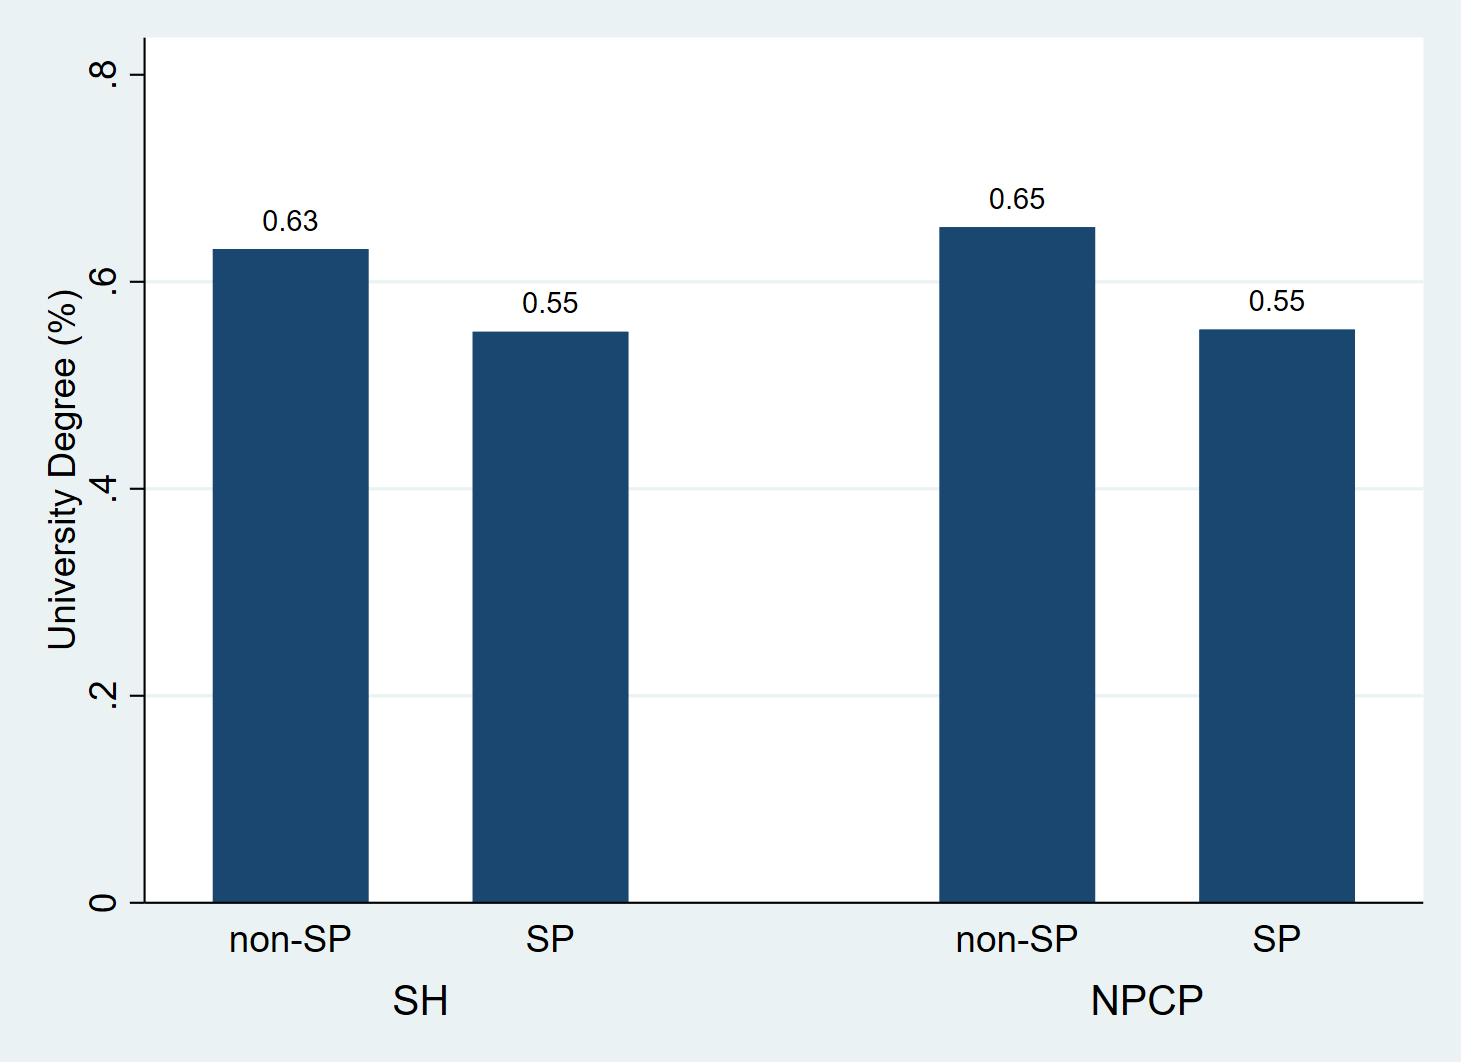
\includegraphics[scale=0.13]{university_sp.png}
        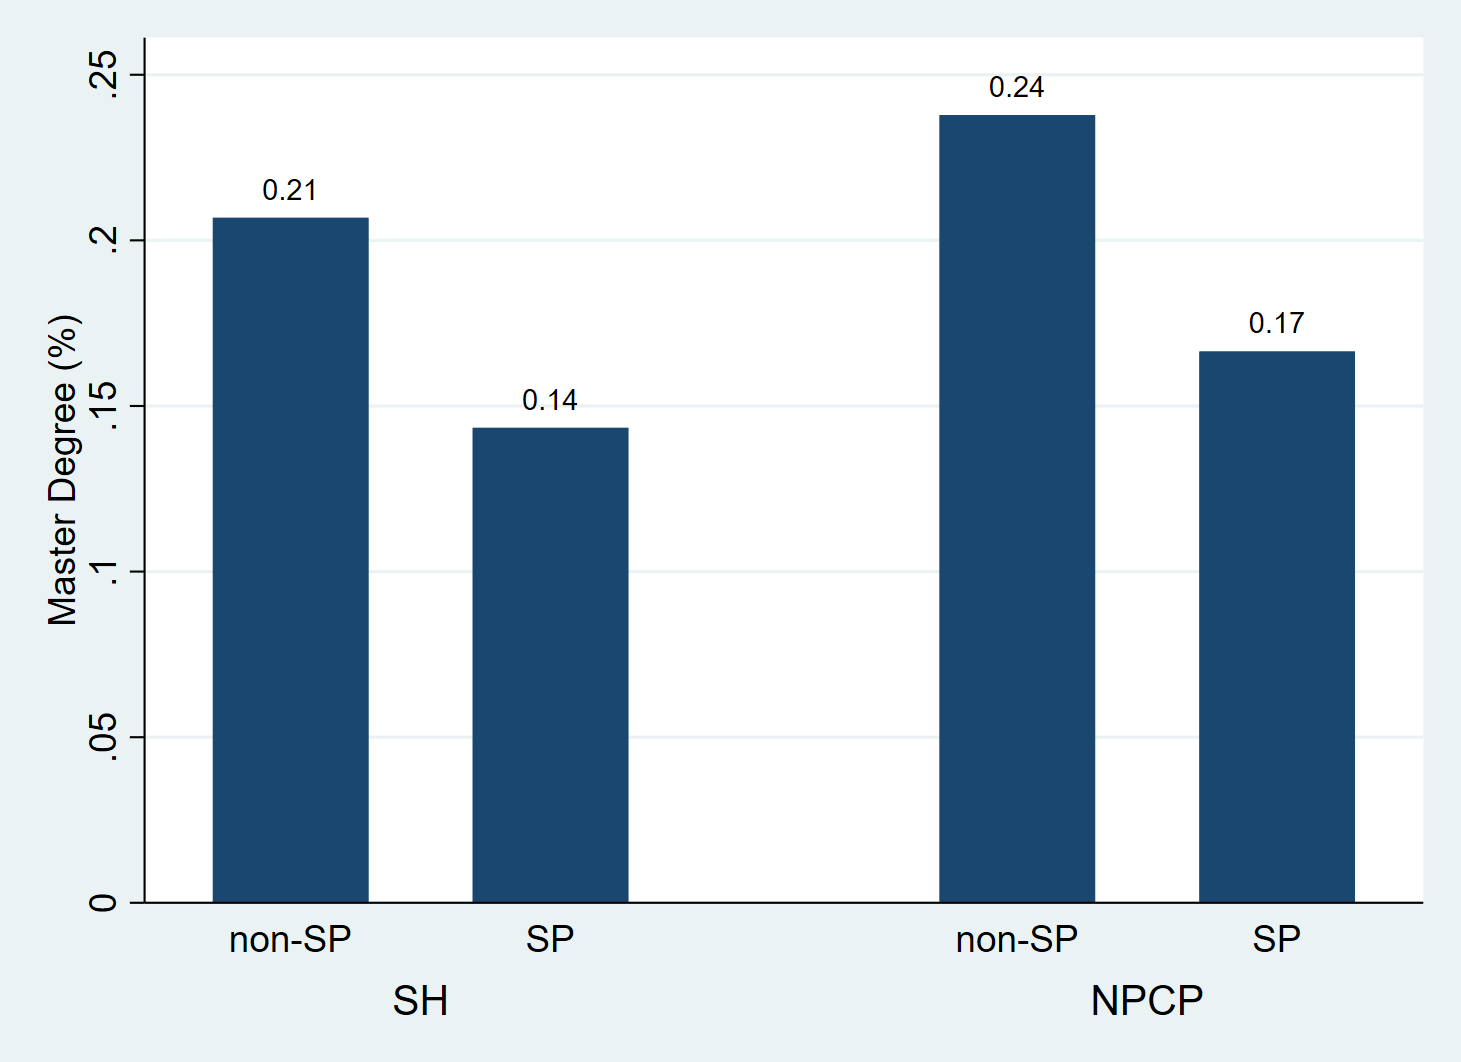
\includegraphics[scale=0.13]{master_sp.png}
        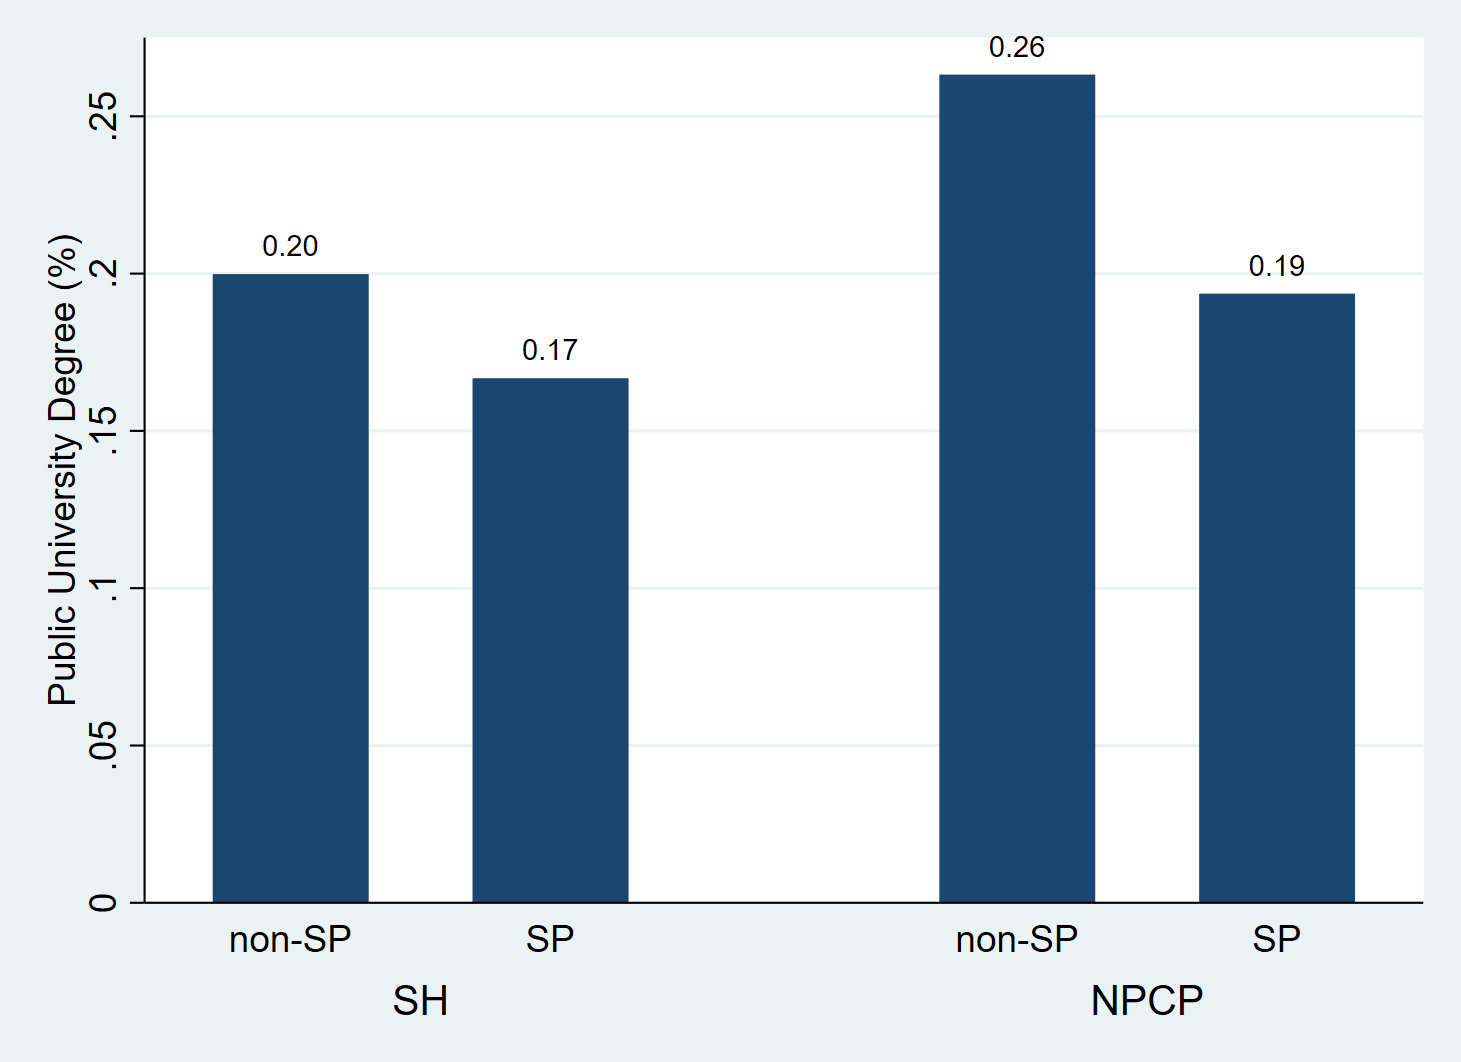
\includegraphics[scale=0.13]{public_sp.png}
    \end{figure}

    Finally, the comprehensive dataset also includes the survey data on their parent and teachers, in which the evaluation and observation on the children in their school age are detaily recorded.  We consider these dataset as the cure to omitted variable bias, so we look at each teacher's data thoroughly and pick every potential confounding variable that either relates to treatment or outcome variable.  Besides, it's worth mentioning that since we want to reduce biasedness, we pay a lot of attention to not include a covariate regarded as \textbf{bad control} by us.  As the following setup is done, we can move forward to the PDS analysis.


\section{Empirical Method} % Second paragraph: what's the assumption and the specification?

    The Post-Double Selection (PDS) method combining causal inference and machine learning is a very powerful and convenient method when we face this kind of huge and comprehensive dataset.  Usually, it's the \textbf{curse of dimensionality} problem we will encounter when we include more covariates and try to reduce the underlying omitted variable bias; however, the PDS method tackle with this problem with introducing Lasso (Least Absolute Shrinkage and Selection Operator) and regression with multiple stages.

    There are two assumptions supporting PDS method: conditional independence assumption and approximate sparsity, and three regression stages in PDS.  The first and second stage use Lasso to conduct regression on different dependent variable, that is, treatment variable and outcome variable, which can be formulated as below

    \begin{align}
    \text{SP}_i = \theta_0 + \sum_{i=1}^n \theta_j X_i^j + \lambda_\theta\sum_{i=1}^n \lvert \theta_j \rvert + \epsilon_i \\
    Y_i         = \eta_0   + \sum_{i=1}^n \eta_j X_i^j   + \lambda_\eta\sum_{i=1}^n \lvert \eta_j   \rvert + \delta_i
    \end{align}

    where the $X^j$ is the covariate we choose from the dataset, and $\{\lambda_\theta,\lambda_\eta\}$ are tuning parameters in the Lasso regression.  After the stages, we will have two different sets of selected covariates, denoted as $\Lambda_\theta,\ \Lambda_\eta$, and their union represents all the potential confounders.  So we can conduct the third stage OLS regression to identify the causal effect in the presence of CIA:

    \begin{align}
        Y_i = \beta_0 + \beta_{\text{PDS}}\text{SP}_i + \sum_{j \,\in\, \Lambda_\theta \cup \Lambda_\eta} \beta_j X_i^j + \epsilon_i
    \end{align}

    After we follow the same analysis process for each group, SH and CP, we obtain the estimated effect and discover the unexpected result which we will show in next part.


\section{Result}

    Accordingly, we perform the three different kinds of regression model, so as to gradually eliminate the omitted variable bias.  The first model is the single variable OLS, which gives us some interpretation of the correlation, the second model is the extension, in which we add some controlled variable related to the student's background; and the last model is the PDS regression, where we put in all the possible confounders and awaits for machine's selection.  We should first show our result on the first outcome variable: university degree

    \begin{center}
    \begin{table}
    \caption{Regression on University for SH and CP group}
    \setlength{\tabcolsep}{0.5mm}
    \begin{tabular}{l*{6}c}
    \toprule
    &\multicolumn{3}{c}{SH} &\multicolumn{3}{c}{CP/NP} \\
    \cmidrule(l){2-4}\cmidrule(l){5-7}
    &\multicolumn{1}{c}{(1)}&\multicolumn{1}{c}{(2)}&\multicolumn{1}{c}{(3)}&\multicolumn{1}{c}{(4)}&\multicolumn{1}{c}{(5)}&\multicolumn{1}{c}{(6)} \\
    &\multicolumn{1}{c}{University}&\multicolumn{1}{c}{University}&\multicolumn{1}{c}{University}&\multicolumn{1}{c}{University}&\multicolumn{1}{c}{University}&\multicolumn{1}{c}{University} \\
    \midrule
    sp          &     -0.0935\sym{***}&     -0.0262         &     -0.0136         &     -0.0340\sym{**} &     -0.0322\sym{**} &     -0.0264\sym{**} \\
                &     (0.000)         &     (0.116)         &     (0.402)         &     (0.011)         &     (0.015)         &     (0.041)         \\
    [1em]
    female      &                     &      0.0187\sym{**} &                     &                     &      0.0198\sym{***}&                     \\
                &                     &     (0.048)         &                     &                     &     (0.004)         &                     \\
    [1em]
    hs\_private  &                     &     -0.0785\sym{***}&     -0.0386\sym{***}&                     &     -0.0474\sym{***}&                     \\
                &                     &     (0.000)         &     (0.000)         &                     &     (0.000)         &                     \\
    [1em]
    hs\_urban    &                     &      0.0459\sym{***}&                     &                     &      0.0466\sym{***}&      0.0124         \\
                &                     &     (0.000)         &                     &                     &     (0.000)         &     (0.159)         \\
    [1em]
    general\_high&                     &       0.607\sym{***}&       0.514\sym{***}&                     &           0         &                     \\
                &                     &     (0.000)         &     (0.000)         &                     &         (.)         &                     \\
    [1em]
    paedu       &                     &      0.0991\sym{***}&      0.0739\sym{***}&                     &      0.0448\sym{***}&      0.0330\sym{***}\\
                &                     &     (0.000)         &     (0.000)         &                     &     (0.000)         &     (0.000)         \\
    [1em]
    PDS\_control  &   &  &  Yes    &  &    &  Yes \\
    &   &      &      &   &      &      \\
    \hline
    \(N\)       &        5230         &        5230         &        5230         &        5766         &        5766         &        5766         \\
    \bottomrule
    \multicolumn{3}{l}{\footnotesize \textit{p}-values in parentheses} & \multicolumn{4}{r}{\footnotesize \sym{*} \(p<0.10\), \sym{**} \(p<0.05\), \sym{***} \(p<0.01\)}\\
    \end{tabular}
    \begin{tablenotes}
        The "PDS control" indicates whether we include covariates to perform PDS.  The number of total covariates we include is 98 for SH group, and 77 for CP group; the number of selected covariates is 22 for SH group, and 8 for CP group.
    \end{tablenotes}
    \end{table}
    \end{center}

    From table 1, the single variable OLS result matches our intuition with a strongly negative correlation between living in single parent family and obtaining university degree in future; however, it also shows that when considering the PDS regression for SH group, the causal relationship is not significant, while for CP group it's significant.  This is the most interesting point in our analysis, because it's very peculiar as we expect the negative causal effect holds for these two different groups, but how does it differ?  We wiil explain when we dig deeper, that is, analyzing the other outcome variables.

    \begin{center}
    \begin{table}
    \caption{Regression on Master for SH and CP group}
    \setlength{\tabcolsep}{0.5mm}
    \begin{tabular}{l*{6}c}
    \toprule
    &\multicolumn{3}{c}{SH} &\multicolumn{3}{c}{CP/NP} \\
    \cmidrule(l){2-4}\cmidrule(l){5-7}
    &\multicolumn{1}{c}{(1)}&\multicolumn{1}{c}{(2)}&\multicolumn{1}{c}{(3)}&\multicolumn{1}{c}{(4)}&\multicolumn{1}{c}{(5)}&\multicolumn{1}{c}{(6)} \\
    &\multicolumn{1}{c}{Master}&\multicolumn{1}{c}{Master}&\multicolumn{1}{c}{Master}&\multicolumn{1}{c}{Master}&\multicolumn{1}{c}{Master}&\multicolumn{1}{c}{Master} \\
    \midrule
    sp          &     -0.0787\sym{***}&     -0.0462\sym{**} &     -0.0405\sym{**} &     -0.0635\sym{***}&     -0.0549\sym{***}&     -0.0465\sym{**} \\
            &     (0.000)         &     (0.011)         &     (0.024)         &     (0.001)         &     (0.005)         &     (0.015)         \\
    [1em]
    female      &                     &     -0.0831\sym{***}&     -0.0597\sym{***}&                     &      -0.111\sym{***}&     -0.0558\sym{***}\\
                &                     &     (0.000)         &     (0.000)         &                     &     (0.000)         &     (0.000)         \\
    [1em]
    hs\_private  &                     &     -0.0649\sym{***}&                     &                     &     -0.0494\sym{***}&                     \\
                &                     &     (0.000)         &                     &                     &     (0.001)         &                     \\
    [1em]
    hs\_urban    &                     &      0.0526\sym{***}&                     &                     &      0.0833\sym{***}&      0.0570\sym{***}\\
                &                     &     (0.000)         &                     &                     &     (0.000)         &     (0.000)         \\
    [1em]
    general\_high&                     &       0.246\sym{***}&       0.156\sym{***}&                     &           0         &                     \\
                &                     &     (0.000)         &     (0.000)         &                     &         (.)         &                     \\
    [1em]
    paedu       &                     &       0.147\sym{***}&       0.129\sym{***}&                     &       0.102\sym{***}&      0.0813\sym{***}\\
            &                     &     (0.000)         &     (0.000)         &                     &     (0.000)         &     (0.000)         \\
    [1em]
    PDS\_control  &   &  &  Yes    &  &    &  Yes \\
    &   &      &      &   &      &      \\
    \hline
    \(N\)       &        4848         &        4848         &        4848         &        5600         &        5600         &        5600         \\
    \bottomrule
    \multicolumn{3}{l}{\footnotesize \textit{p}-values in parentheses} & \multicolumn{4}{r}{\footnotesize \sym{*} \(p<0.10\), \sym{**} \(p<0.05\), \sym{***} \(p<0.01\)}\\
    \end{tabular}
    \begin{tablenotes}
        The "PDS control" indicates whether we include covariates to perform PDS.  The number of total covariates we include is 98 for SH group, and 77 for CP group; the number of selected covariates is 11 for SH group, and 8 for CP group.
        % puclic: SH is 16, CP is 20
    \end{tablenotes}
    \end{table}
    \end{center}

    In table 2, we see all the coefficient are significant under 1\% significant level, which indicates the effect is very strong.  As the PDS regression result shows, living in single parent family will reduce the probability of obtaining master degree by 4\% and 4.6\%, respectively for SH and CP group.  We regard the impact as very prodigious and suggest that the underlying channels, economics situation and mental support, play a crucial role in the process.

    \begin{center}
    \begin{table}
    \caption{Regression on Public University for SH and CP group}
    \setlength{\tabcolsep}{0.5mm}
    \begin{tabular}{l*{6}c}
    \toprule
    &\multicolumn{3}{c}{SH} &\multicolumn{3}{c}{CP/NP} \\
    \cmidrule(l){2-4}\cmidrule(l){5-7}
    &\multicolumn{1}{c}{(1)}&\multicolumn{1}{c}{(2)}&\multicolumn{1}{c}{(3)}&\multicolumn{1}{c}{(4)}&\multicolumn{1}{c}{(5)}&\multicolumn{1}{c}{(6)} \\
    &\multicolumn{1}{c}{Public}&\multicolumn{1}{c}{Public}&\multicolumn{1}{c}{Public}&\multicolumn{1}{c}{Public}&\multicolumn{1}{c}{Public}&\multicolumn{1}{c}{Public} \\
    \midrule
    sp          &     -0.0229         &     0.00651         &     0.01000         &     -0.0768\sym{***}&     -0.0739\sym{***}&     -0.0443\sym{**} \\
            &     (0.212)         &     (0.705)         &     (0.553)         &     (0.000)         &     (0.000)         &     (0.020)         \\
    [1em]
    female      &                     &      0.0157         &                     &                     &     -0.0319\sym{**} &                     \\
                &                     &     (0.154)         &                     &                     &     (0.012)         &                     \\
    [1em]
    hs\_private  &                     &      -0.117\sym{***}&     -0.0675\sym{***}&                     &      -0.182\sym{***}&     -0.0860\sym{***}\\
                &                     &     (0.000)         &     (0.000)         &                     &     (0.000)         &     (0.000)         \\
    [1em]
    hs\_urban    &                     &      0.0591\sym{***}&                     &                     &       0.131\sym{***}&      0.0968\sym{***}\\
                &                     &     (0.000)         &                     &                     &     (0.000)         &     (0.000)         \\
    [1em]
    general\_high&                     &       0.229\sym{***}&       0.184\sym{***}&                     &           0         &                     \\
                &                     &     (0.000)         &     (0.000)         &                     &         (.)         &                     \\
    [1em]
    paedu       &                     &       0.123\sym{***}&      0.0978\sym{***}&                     &       0.110\sym{***}&      0.0641\sym{***}\\
            &                     &     (0.000)         &     (0.000)         &                     &     (0.000)         &     (0.000)         \\
    [1em]
    PDS\_control  &   &  &  Yes    &  &    &  Yes \\
    &   &      &      &   &      &      \\
    \hline
    \(N\)       &        5027         &        5027         &        5027         &        5576         &        5576         &        5576         \\
    \bottomrule
    \multicolumn{3}{l}{\footnotesize \textit{p}-values in parentheses} & \multicolumn{4}{r}{\footnotesize \sym{*} \(p<0.10\), \sym{**} \(p<0.05\), \sym{***} \(p<0.01\)}\\
    \end{tabular}
    \begin{tablenotes}
        The "PDS control" indicates whether we include covariates to perform PDS.  The number of total covariates we include is 98 for SH group, and 77 for CP group; the number of selected covariates is 16 for SH group, and 20 for CP group.
    \end{tablenotes}
    \end{table}
    \end{center}

    Now let's look at table 3, where the PDS regression result looks similar to the first table.  Compared with significantly negative impact for CP group, it's noticeable the impact nearly exist for SH group.  So why is there an unneglected difference between these two group?  Since the only different characteristic for these groups are born year, we suggest the difference might by attributed to the Taiwan Education Reform in 2000s, when the number of university skyrocketed in order to increase the general education degree of people.  
    
    Although the reform made competition for children to get into university be reduced; however, we thinks the policy may enlarge the gap between those with good/bad economic condition, or in other words, living in single parent/nuclear family.  The policy may do provide more opportunities for children to enter the university, but failing to cover the money shortage of those with bad economic condition, as a consequence, they would tend to suspend their educational investment after high school and enter labor market for finding work.  This sounds like a plausible story, with some evidence, we can make the argument more credible.

\section{Discussion and Conclusion}

    Overall, we find out that single parent family has the significant negative effect on academic degrees, especially in master degree. We also observe the different impact of single parent family. However, the channel is still unknown. The different effects between two groups might be related to the economic conditions of the students. 

    To confirm that the difference between SH and CP group is truely induced by family's economic background, we show another dependent variable -- $work\_year$ further. The variable $work\_year$ is defined as how many years these students enter the labor market when they are 25 years old. If single parent families do influence the students' economic situation, it is possible that students in single parent family will enter the labor market earlier, rather than getting the higher educational degree. Thus, we simply run the regression of single parent family on working year.

    In table 4, the single regression with some control variables we selected shows that single parent families have significant effect on CP group, while it is not significant in SH group, which directly confirm our suppose about bad economic conditions in single parent families. Although the scale is only 0.2 year, we believe single parent families somehow force their children to enter the labor market earlier than general students, which might influence their highest level of education.

    Besides, our results is consistent to the previous paper.  \citet{Luoh2004}  also prove the educational reform around 2000s does not benefit some economic vulnerable groups. He analyzes the probability change of entering Taiwan universities. Due to the educational reform in 1987, the amount of university in Taiwan abruptly increased. The total number of universities was 60 in 1995, but 135 in 2001, which allowed more students to attend the university.  \citet{Luoh2004} point out that when the proportion of school attendance is low, the increase of school opportunities will increase the influence of family background on the probability of individual school attendance, which means students from bad economic backgrounds family will have more negative impact on the probability of attaining the bachelor degree. 
   
    In our cases, single parent family do have some economic situation. The negative effect of single parent family is not really obvious until the educational reform enhance the total probability of entering universities,which somehow croud out the children from single parent family, making the coefficient of CP group to be significant.
    
    \begin{center}
        \begin{table}
        \caption{Regression on Working Year for SH and CP group}
        \setlength{\tabcolsep}{0.5mm}
        \begin{tabular}{l*{4}c}
        \toprule
        &\multicolumn{2}{c}{SH} &\multicolumn{2}{c}{CP/NP} \\
        \cmidrule(l){2-3}\cmidrule(l){4-5}
        &\multicolumn{1}{c}{(1)}&\multicolumn{1}{c}{(2)}&\multicolumn{1}{c}{(3)}&\multicolumn{1}{c}{(4)}\\
        &\multicolumn{1}{c}{Work\_year}&\multicolumn{1}{c}{Work\_year}&\multicolumn{1}{c}{Work\_year}&\multicolumn{1}{c}{Work\_year}\\
        \midrule
        sp          &       0.257\sym{**} &       0.153         &       0.214\sym{***}&       0.200\sym{***}\\
                    &     (0.032)         &     (0.180)         &     (0.006)         &     (0.009)         \\
        [1em]
        female      &                     &      0.0312         &                     &       0.437\sym{***}\\
                    &                     &     (0.675)         &                     &     (0.000)         \\
        [1em]
        hs\_private  &                     &       0.380\sym{***}&                     &       0.139\sym{**} \\
                    &                     &     (0.000)         &                     &     (0.010)         \\
        [1em]
        hs\_urban    &                     &      -0.112\sym{*}  &                     &      -0.167\sym{***}\\
                    &                     &     (0.093)         &                     &     (0.000)         \\
        [1em]
        general\_high&                     &      -1.012\sym{***}&                     &           0         \\
                    &                     &     (0.000)         &                     &         (.)         \\
        [1em]
        paedu       &                     &      -0.400\sym{***}&                     &      -0.290\sym{***}\\
                    &                     &     (0.000)         &                     &     (0.000)         \\
        [1em]
        \_cons      &       2.959\sym{***}&       3.465\sym{***}&       2.940\sym{***}&       2.815\sym{***}\\
                    &     (0.000)         &     (0.000)         &     (0.000)         &     (0.000)         \\
        \hline
        \(N\)       &        2685         &        2685         &        3548         &        3548         \\
        \hline\hline
        \multicolumn{2}{l}{\footnotesize \textit{p}-values in parentheses} & \multicolumn{3}{r}{\footnotesize \sym{*} \(p<0.10\), \sym{**} \(p<0.05\), \sym{***} \(p<0.01\)}\\
        \end{tabular}
        \begin{tablenotes}
            We only run the simple regression with some control variables since the PDS method would drop most of the samples. The data quality doesn't allow us to utilize PDS method in this case.
        \end{tablenotes}
        \end{table}
        \end{center}
    
   





% Remove or comment out the next two lines if you are not using bibtex.
\bibliographystyle{aea}
\bibliography{BibFile}

% The appendix command is issued once, prior to all appendices, if any.
\appendix



\bibliographystyle{unsrt}
\bibliography{reference}



\end{document}

